\subsection{Knowledge Engineering}\label{sec:ke}
Initially, the solutions for NLP problems were all based on a common approach of identifying better features to represent the text data. These features are identified based on the domain expertise and are very specific to the problem they are applied in. This category of techniques can be classified as the techniques which requires a lot of domain knowledge in order to achieve good results. They don't need a lot of training data in order to gain good performance but the performance gets saturated after some amount of data, i.e., the performance doesn't increase with the increase in training data. We group these methods into two categories:

\begin{enumerate}
    % \item Rule Based
    \item Case Based Reasoning
    \item Machine Learning
\end{enumerate}

% \subsubsection{Rule Based}
% The techniques which requires a pre-defined set of rules to identify the matches and solve the problem.

% \paragraph{Syntax driven} It takes a syntax driven approach to semantic 

% is the approach where syntax

% \paragraph{Lexicon approach} requires a set of dictionary/lexicon defined in order to identify 

% \paragraph{Ontology based}

% \paragraph{Linguistic Features}\label{sec:ling_ftrs}
% A sentence can be processed to extract parts of speech, noun chunks, and entities. Some of the features that can be generated afterwards are as follows:

% \begin{enumerate}
%     \item word length: number of tokens in sentence.
%     \item word length 2: number of words in sentences with stopwords removed.
%     \item has modal: indicates if the sentence contains a modal.
%     \item num of modals: number of modals in sentence.
%     \item modal position: average position of modal verbs in a sentence (-1 if none).
%     \item num of entities: number of named entities in sentence.
%     \item m trigger word: checks if the sentence contains any mandatory term (true/false).
%     \item m trigger position: average position of mandatory terms in sentence ([0.0,1.0] interval and -1 if none).
%     \item n trigger word: checks if the sentence contains any non-mandatory term (true/false).
%     \item n trigger position: average position of non-mandatory terms in sentence ([0.0,1.0] interval and -1 if none).
% \end{enumerate}


\subsubsection{Case Based Reasoning}
Case Based Reasoning is a sub-field of Artificial Intelligence which solves the problems on the basis of modelling real word intuition that similar problem have similar solutions. When we see a new problem in our real life, we try to map it to our previous experience of similar problems and solve it taking similar approach. In CBR as well, we retrieve the problems similar to the new one and use the similar kind of approach to solve it using the solutions stored in knowledge base (KB). In the KB, we store these cases in a pair of problem and solution. A CBR cycle generally have 4 steps as defined in \cite{aamodt1994case}. Fig. \ref{fig:cbr_4r} shows the 4Rs of a CBR cycle.

\begin{enumerate}
    \item RETRIEVE the cases similar to the new problem.
    \item REUSE the information or solution for similar cases to solve the new one.
    \item REVISE the new proposed solution.
    \item RETAIN the useful information of new case in the KB for future use.
\end{enumerate}

\begin{figure}
    \centering
    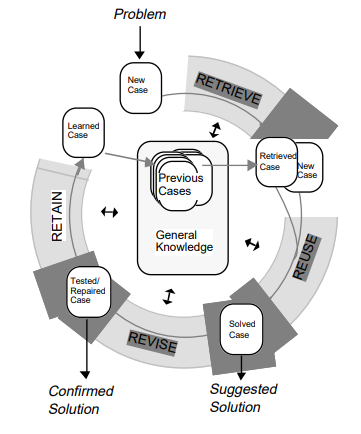
\includegraphics[width=0.45\textwidth]{images/cbr_4r.png}
    \caption{4Rs of a CBR Cycle \cite{aamodt1994case}}
    \label{fig:cbr_4r}
\end{figure}

\paragraph{k-Nearest Neighbours (k-NN)} One of the most common CBR algorithm is k-Nearest Neighbour which computes the distance between the new case and all other previous cases. Then the k cases with the minimum distance are selected as the similar cases and there solution is used to make decision for the new case's solution. k-NN uses the euclidean distance to measure distance between two cases. The distance between two cases $c_{i}$ and $c_{j}$ is given in \cref{eq:knn}

\begin{equation}
    \label{eq:knn}
        Dist(c_{i}, c_{j}) = \sqrt{\sum_{v=1}^{n} (c_{iv}-c_{jv})_{2}}
\end{equation}

where v is the dimension of problem in the case. This technique is also referred as lazy learning sometimes as it makes observation on the previous knowledge every time a new query is given rather than trying to learn a general model for knowledge base in training and using that model to answer a query when asked.

\paragraph{Textual Case-Baed Reasoning (TCBR)}
TCBR is a bit different from general CBR in terms of representation of problem and solution of the cases, altough the 4Rs of a CBR cycle holds true here as well. In TCBR, some or whole part of the previous cases are stored in textual form and we aim to solve the problem for new cases with the help of these textual knowledge sources in automated way \cite{weber2005textual}. The cases are stored in two sets namely, problem set and solution set. In TCBR, the focus is on defining a good representation of these sets and then finding a way to evaluate these representations.

\paragraph{Text Representation}
Representing cases in text CBR is a trivial task as there is no standard representation defined that can work for every problem. But one of the most commonly used representation is using bag of words \cite{10.5555/646268.684025}. In this representation, a sentence is is broken into tokens which are essentially the words of the sentence and their appearance is different manner is used as the features. One of the drawback of using this technique is that we loose the sequence information as it is lost during the tokenisation process.

Another common way of representing texts is by grouping them into attribute-value pairs to generate feature vectors, where attributes are decided based on the domain and values are the pieces of text from the case base. This approach works for maximum cases but the attributes differ from problem to problem as they are domain specific. An example of attribute-value pair can be a case storing the information of a student with attributes such as \textit{Student Name - Ashish Upadhyay} and \textit{School - Computing Science and Digital Media}.

There are other examples of case representation as well, like used in popular CBR framework jCOLIBRI where cases are stored in tree structure where each case is treated as an individual capable of containing other individuals and thus forming the tree structure.

\paragraph{Evaluation}
After the representation of text cases is done, we need to evaluate it by measuring the similarity or alignment between cases problem and solution set. A good representation will provide much better alignment between cases than a bad representation.

Two most common ways of measuring the similarity can be local alignment and global alignment \cite{raghunandan2008evaluation}. The local alignment measure uses the alignment of each case with its neighbourhood and then aggregates the values for all cases to find the alignment for whole case base whereas the global method measures the alignment value for whole case base as one single entity.

\subsubsection{Machine Learning}
Machine Learning is another subset of Artificial Intelligence which learns a general distribution of the previous experience by using the training data and then uses the learned distribution to predict the answer a new problem. In Machine Learning, we mostly use sparse representation of the problems of a case and use statistical algorithms to learn the general distribution of training set.

The difference of machine learning approach from case-based approach is that machine learning, the distribution is learned during the training process and that learning is used to answer a query during test or deployment phase whereas in case-based reasoning, the case-base is searched to retrieve the similar cases every time a query is asked in order to answer it.

Some of the representations and learning algorithms used in machine learning are briefly discussed here. Term Frequency (TF), Term Frequency-Inverse Document Frequency (TFIDF) and Linguistic Features are some of the most common feature representations, whereas Support Vector Machines, Random Forest and Naive Bayes are some of the commonly used learning algorithms.

\paragraph{Term Frequency Vectors}
This feature vector is used to represent a document by assembling a vector of the frequency of the terms contained in the document. Here we first extract all the terms from the  documents and  create a corpus dictionary of all the terms. Then the frequency of  the terms from each document is calculated to generate the vector representing that document. The vectors can be presented as a document term matrix, where each row  is a document vector and each column represent a term from the corpus dictionary.

To calculate the term frequency we apply the following formula: 
\begin{equation}
tf(t) = m/k
\end{equation}
Where, the number of times term $t$ has appeared in a document is represented by $m$ and the total number of terms in the document is denoted by $k$.

Let's understand this with an example. Suppose, in our training dataset we have $N$ documents. After extracting all the terms from the documents and creating the corpus, we get total $M$ unique terms. So our count vector will be a $N\times M$ matrix where every row is a document and every column is a term from the corpus. So each document is represented as a $1\times M$ vector.

For example, let's say we have two documents:
\begin{center}
	D1: The valve must be coloured black.\\
	D2: The wire must remain covered.
\end{center}
Thus the corpus dictionary created would look like this:
\begin{center}
	[`be', `black', `coloured', `covered', `must', `remain', `the', `valve', `wire']
\end{center}
So, the count vector for this example would be a $2\times 10$ matrix and can be represented as follows:
\begin{table}
	\centering
	\caption{TF vector representation.}\label{tab2}
	\begin{tabular}{|l|l|l|l|l|l|l|l|l|}
		\hline
		be & black & coloured & covered & must & remain & the & valve & wire\\
		\hline
		0.166 & 0.166 & 0.166 & 0 & 0.166 & 0 & 0.166 & 0.166 & 0\\
		0 & 0 & 0 & 0.166 & 0.166 & 0.166 & 0.166 & 0 & 0.166\\
		\hline
	\end{tabular}
\end{table}


\paragraph{Term Frequency - Inverse Document Frequency Vector}\label{sec:tfidf}
This feature vector is different from the TF vector in a way where it takes into account the occurrence of a term in whole corpus not just the occurrence of that term in a document. The intuition behind this is to reflect how important a term is to document by giving popular terms a low weight and rare terms a higher weight. The TF-IDF can be divided into two parts: term frequency and inverse document frequency. 

For calculating term frequency, we can use the same method discussed above in Equation 1.

Then we calculate the inverse document frequency by using the following formula.
\begin{equation}
idf(t) = log(N/n)
\end{equation}

Where $n$ is the number of documents term $t$ has appeared and $N$ is the number of documents.

So, the formula to calculate $tfidf$ is given as:
\begin{equation}
tfidf(t) = tf*idf = (m/k)*\log(N/n)
\end{equation}

That's why in this way,  terms like $the, is, a$ are heavily penalized.  Rarely occurring terms in a corpus get high $idf$ score. To compare with the TF representation, let's take the same example discussed in previous section. So, the $tfidf$ for term $the$ from document $D1$ can be calculated as:
\begin{center}
	$tf = 2/8 = 0.25$\\
	$idf = \log(2/2) = 0$\\
	$tfidf = 0.25*0 = 0$
\end{center}

\paragraph{Linguistic Features}\label{sec:ling_ftrs}
A sentence can be processed to extract parts of speech, noun chunks, and entities. Some of the features that can be generated afterwards are as follows:

\begin{enumerate}
    \item word length: number of tokens in sentence.
    \item word length 2: number of words in sentences with stopwords removed.
    \item has modal: indicates if the sentence contains a modal.
    \item num of modals: number of modals in sentence.
    \item modal position: average position of modal verbs in a sentence (-1 if none).
    \item num of entities: number of named entities in sentence.
    % \item m trigger word: checks if the sentence contains any mandatory term (true/false).
    % \item m trigger position: average position of mandatory terms in sentence ([0.0,1.0] interval and -1 if none).
    % \item n trigger word: checks if the sentence contains any non-mandatory term (true/false).
    % \item n trigger position: average position of non-mandatory terms in sentence ([0.0,1.0] interval and -1 if none).
\end{enumerate}

\paragraph{Random Forest}
Random forest \cite{breiman2001random} is an ensemble algorithm of both multiple decision trees used for classification or regression. It initialises a forest of many random decision trees by applying sampling on the train data. Every tree initialised in the forest uses subset or the random samples of number of observations available as well as only taking the random sample of features from the dataset.

% Suppose, you have a dataset of $n$ observations and $k$ features, i.e., a matrix of $n\times k$ for training and you wish to grow 100 trees in your forest, then every tree in the forest will take random $n_0$ observations and $k_0$ features for training where $n_0 < n$ and $k_0 < k$.

\paragraph{Support Vector Machine}\label{svm}
A Support Vector Machine (SVM) formally defined by a separating hyperplane is a discriminative classifier that can be used to classify both linear and non-linear data \cite{vapnik2013nature}. A Support Vector Machine gives an optimal hyperplane dividing the training examples into different classes. For a multi-class classification where number of classes is more than two, an SVM iteratively finds the optimal plane by diving the problem into one-vs-all. In every iteration, it takes one class as positive and rest of the classes as negative and finds the hyperplane dividing that data combination. SVM can be very slow for large datasets as the time complexity is proportional to the square of features used.

\paragraph{Naive Bayes}
Naive Bayes is an algorithm based on Bayes theorem which models the distribution of a class using independent conditional probability \cite{han2011data}. It is very fast and scalable and can be applied to various problems with bigger datasets in text mining.

